\documentclass[11pt]{article}
\usepackage{../template}

\graphicspath{ {./img/} }
\addbibresource{../references.bib}

\begin{document}

\section{Modeling LTS: Control TTX}

\textbf{What do we know?}

\begin{align}
    \min_{\mathbf{x}_0,\, T} & \quad J({\mathbf{x}_0,\, T})\\
    \text{with, } & \quad J = \left\| \mathbf{x}(T; \mathbf{x}_0 ,\boldsymbol\theta) - \mathbf{x}_0 \right\|
\end{align}

\begin{itemize}
    \item The initial uprize is potentially caused by T-type Ca current, as no activity
    is found in the T-Type Ca channel KD scenario (Figure \ref{fig_ttx_t_kd})
    
    \item Fast hyperpolarizing current when the membrane potential reaches specific value (Figure \ref{fig_ttx_control})
    By rough approximation, the timescale of the strong hyperpolarization is around 100ms
    
    \item Slightly reduced bursting frequency in T-type KD neurons, as well as increased resting membrane
    potential (by approximately 5 mV)

    \begin{figure}[H]
        \centering
        % First row
        \begin{subfigure}[t]{0.45\textwidth}
            \centering
            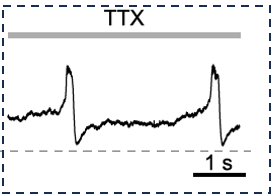
\includegraphics[width=\textwidth]{./img/2025_01_23/control_ttx.png}
            \caption{Recording of membrane potential after application of TTX in control flies}
            \label{fig_ttx_control}
        \end{subfigure}
        \hfill
        \begin{subfigure}[t]{0.45\textwidth}
            \centering
            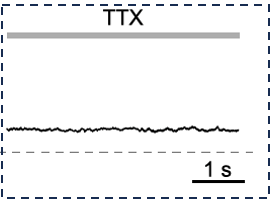
\includegraphics[width=\textwidth]{./img/2025_01_23/t_type_KD.png}
            \caption{Recording of membrane potential after application of TTX in T-type Ca channel KD flies}
            \label{fig_ttx_t_kd}
        \end{subfigure}
        \caption{}
    \end{figure}
\end{itemize}


Generally, subthreshold oscillations might have various different origins. Minimal models can be
constructed with
\begin{itemize}
    \item T-Type and Leak channels
    \item T-Type and Noninactivating hyperpolarizing channels
    \item T-Type and Inactivating hyperpolarizing channels
    \item T-Type and hyperpolarizing Ca gated channels
\end{itemize}

\begin{itemize}

    
    

    \begin{figure}[H]
        \centering
        % First row
        \begin{subfigure}[t]{0.48\textwidth}
            \centering
            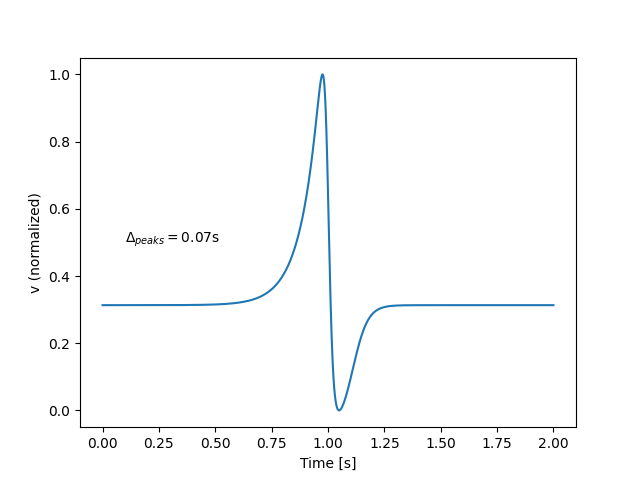
\includegraphics[width=\textwidth]{./img/2025_01_23/ttx_rough_estimate.png}
            \caption{Rough estimate (a guessed function) for the observed LTS after TTX}
            \label{fig_lts_rough_estimate}
        \end{subfigure}
        \hfill
        \begin{subfigure}[t]{0.48\textwidth}
            \centering
            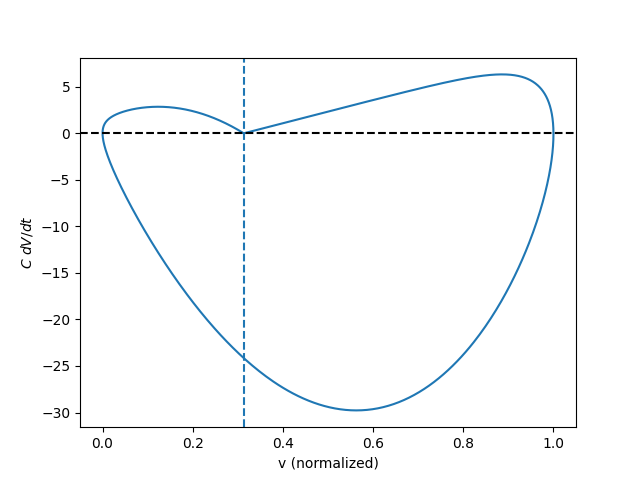
\includegraphics[width=\textwidth]{./img/2025_01_23/ttx_rough_estimate_v_dvdt_phase.png}
            \caption{Membrane potential versus its rate of change for the guessed function}
            \label{fig_lts_rough_estimate_v_dvdt}
        \end{subfigure}
        \caption{}
    \end{figure}

    
    
    \item What can cause the strong hyperpolarization?
    \begin{itemize}
        \item \textbf{(\textcolor{red}{X}) Noninactivating channel (e.g. Slow K current (Ks))}
        
        No, because the current is very strong. The time constant of the activation variable is still
        quite fast (Figre \ref{fig_ks_time_constant}).
        \begin{enumerate}
            \item If the activation threshold is lower than the peak, it would have affected the phase of the
            oscillation, when T-Type channels are activated;
            \item If the activation threshold is around the peak, it would have deinactivated fast and would not
            have caused the membrane potential to reach its trough.
        \end{enumerate} 
        (\textbf{\textcolor{green}{\ding{52}}}) However, it can still cause the small drop seen on top of the peak
        in Figure \ref{fig_ttx_control} (\textcolor{red}{see also Fig. for the simulation results.})
        
        \item \textbf{(\textcolor{orange}{?}): Inactivating channel (e.g. Fast K current (Kf))}
        
        \item \textbf{(\textcolor{orange}{?}): Ligand gated hyperpolarizing currents (e.g. Ca activated K channel)}
        
        As the uprize of the membrane potential is potentially mediated through influx of calcium, the negative
        feedback in the modulation of the membrane potential can be cased by Ca activated hyperpolarizing channels,
        such as Ca gated K channels.

    \end{itemize}
\end{itemize}

\begin{figure}[H]
    \centering
    \begin{subfigure}[t]{0.48\textwidth}
        \centering
        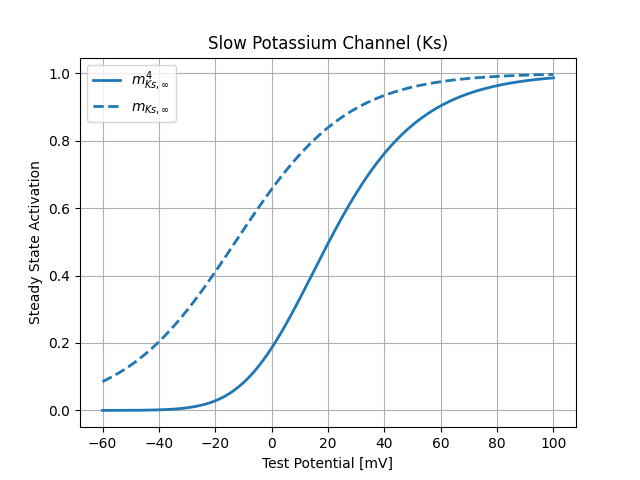
\includegraphics[width=\textwidth]{./img/2025_01_23/Ks_channel_steady_state_activation.png}
        \caption{Steady state activation}
        \label{fig_ks_steady_state_activation}
    \end{subfigure}
    \hfill
    \begin{subfigure}[t]{0.48\textwidth}
        \centering
        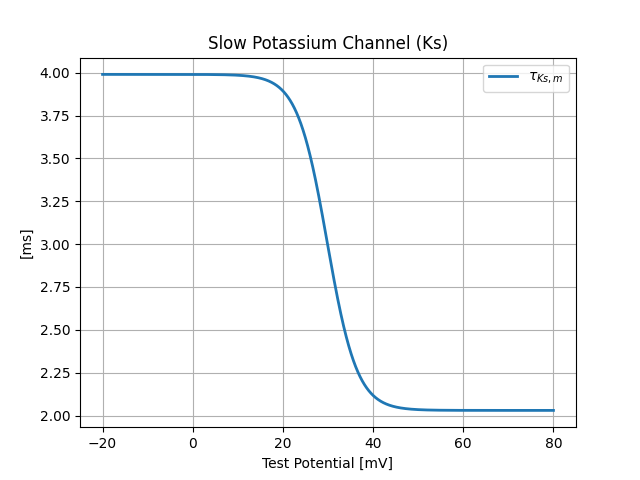
\includegraphics[width=\textwidth]{./img/2025_01_23/Ks_channel_tau_m.png}
        \caption{Activation time constant}
        \label{fig_ks_time_constant}
    \end{subfigure}

    \caption{Kinetiks of Ks channel (parameters taken from \parencite{gunayDistalSpikeInitiation2015})}
\end{figure}


\begin{figure}[H]
    \centering
    \begin{subfigure}[t]{0.48\textwidth}
        \centering
        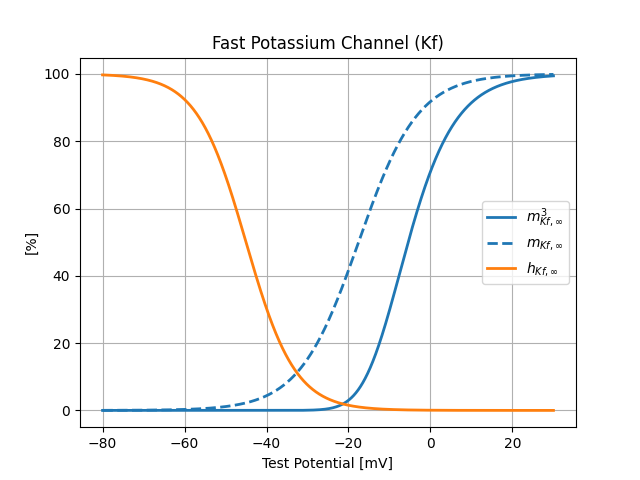
\includegraphics[width=\textwidth]{./img/2025_01_23/Kf_steady_state_variables.png}
        \caption{Steady state activation}
        \label{fig_kf_steady_state_activation}
    \end{subfigure}
    \hfill
    \begin{subfigure}[t]{0.48\textwidth}
        \centering
        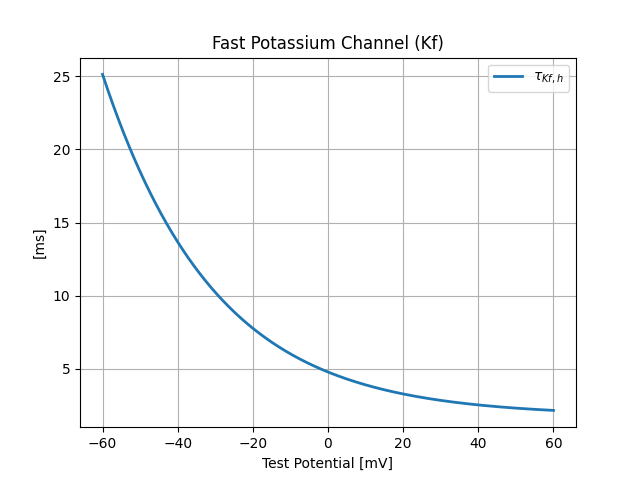
\includegraphics[width=\textwidth]{./img/2025_01_23/Kf_tau_h.png}
        \caption{Inactivation time constant}
        \label{fig_kf_inactivation_time_constant}
    \end{subfigure}
    \hfill
    \begin{subfigure}[t]{0.48\textwidth}
        \centering
        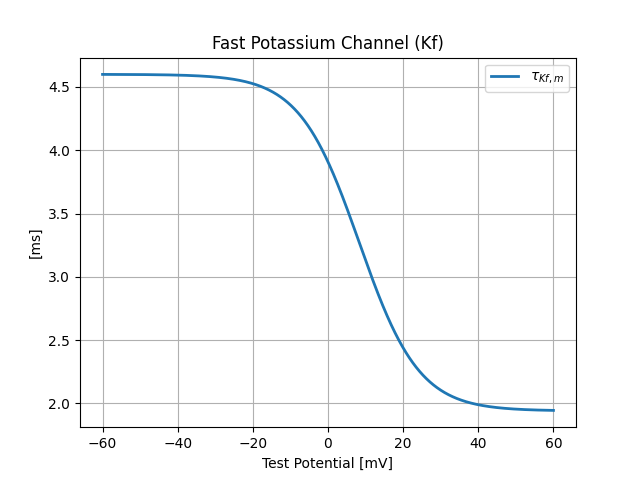
\includegraphics[width=\textwidth]{./img/2025_01_23/Kf_tau_m.png}
        \caption{Activation time constant}
        \label{fig_kf_activation_time_constant}
    \end{subfigure}

    \caption{Kinetiks of Kf channel (parameters taken from \parencite{gunayDistalSpikeInitiation2015})}
\end{figure}

\printbibliography

\end{document}